\documentclass{beamer}
\mode<presentation>
{
  \usetheme{Singapore}
  % oder ...
  %\usecolortheme{lily}
  \setbeamercovered{transparent}
  % oder auch nicht
}

\usepackage[german]{babel}
% oder was auch immer

\usepackage[latin1]{inputenc}
% oder was auch immer

\usepackage{listings}
\usepackage{graphicx}

\usepackage{times}
\usepackage[T1]{fontenc}
% Oder was auch immer. Zu beachten ist, das Font und Encoding passen
% m�ssen. Falls T1 nicht funktioniert, kann man versuchen, die Zeile
% mit fontenc zu l�schen.

\usepackage{url}

\usepackage{ulem}

\title[JMeter]{Apache JMeter}

%\subtitle
%{} % (optional)

\author{Fabian Bieker}

\date%[Kurzversion des Anlass] % (optional)
{26. Januar 2010}
%{\today}

\subject{Apache JMeter}
% Dies wird lediglich in den PDF Informationskatalog einf�gt. Kann gut
% weggelassen werden.


% Falls eine Logodatei namens "university-logo-filename.xxx" vorhanden
% ist, wobei xxx ein von latex bzw. pdflatex lesbares Graphikformat
% ist, so kann man wie folgt ein Logo einf�gen:

%\pgfdeclareimage[width=3cm]{logo}{b4f_logo}
%\logo{\pgfuseimage{logo}}

% Folgendes sollte gel�scht werden, wenn man nicht am Anfang jedes
% Unterabschnitts die Gliederung nochmal sehen m�chte.
\AtBeginSection[]
{
  \begin{frame}<beamer>
    %\frametitle{Agenda}
    \tableofcontents[current,currentsection]
  \end{frame}
}

% Falls Aufz�hlungen immer schrittweise gezeigt werden sollen, kann
% folgendes Kommando benutzt werden:

%
% TODO: human spellchecker
%
\begin{document}

\begin{frame}
  \titlepage
  \begin{figure}
    \centering
    
\includegraphics[scale=0.6]{screen/jmeterLogo.eps}	  
  \end{figure}
\end{frame}

\begin{frame}
  \frametitle{Agenda}
  \tableofcontents
\end{frame}

\begin{frame}
\center{\bf{Fragen? Dann fragt ...}}
\end{frame}

\begin{frame}
  \frametitle{Einleitung}
  \begin{itemize}
   \item Warum Lasttests?
   \item Warum JMeter? \pause
    \begin{itemize}
     \item Flexibel
	 \item Java, leicht erweiterbar
     \item Apache 2.0 Lizenz
     \item Nicht zu langsam
    \end{itemize}
  \end{itemize}
\end{frame}

\begin{frame}
  \frametitle{Grundlagen Lasttests}
  \begin{itemize}
   \item Latenz \& Antwortzeit
   \item Durchsatz
   \item Standardabweichung (Jitter)
   \item I.d.R. misst man den Lastgenerator mit!
  \end{itemize}
\end{frame}

\begin{frame}
  \frametitle{Grundlagen Lasttests}
	s. ``Release It'' - Chap. 8
\end{frame}

\begin{frame}
Stellt JMeter auf englisch um (``Optionen''). Die deutsche Lokalisierung ist
unertr�glich.
\end{frame}

\begin{frame}
  \frametitle{JMeter Konzepte}
  \begin{itemize}
   \item Testpl�ne
   \item Komponenten
   \item Scoping
  \end{itemize}
\end{frame}

\begin{frame}
  \frametitle{JMeter Komponenten}
  \begin{itemize}
   \item Thread Groups
   \item Sampler und Listener
   %\item Configuration Elements
   \item Logic Controller
   \item Assertions
   \item ...
  \end{itemize}
\end{frame}


\section{Simpler HTTP-Testplan}
\begin{frame}
  \frametitle{Thread Group}
  \begin{itemize}
   \item F�hrt For-Schleife mit $n$ Threads aus \pause
   \item JMeter erzeugt Komponenten-Instanzen aus Testplan
   \item Jeder Thread tut etwas mit seinen Instanzen
   \begin{itemize}
      \item z.B. HTTP-Request senden
    \end{itemize}
  \end{itemize}
\end{frame}

\begin{frame}
  \begin{figure}
    \centering
    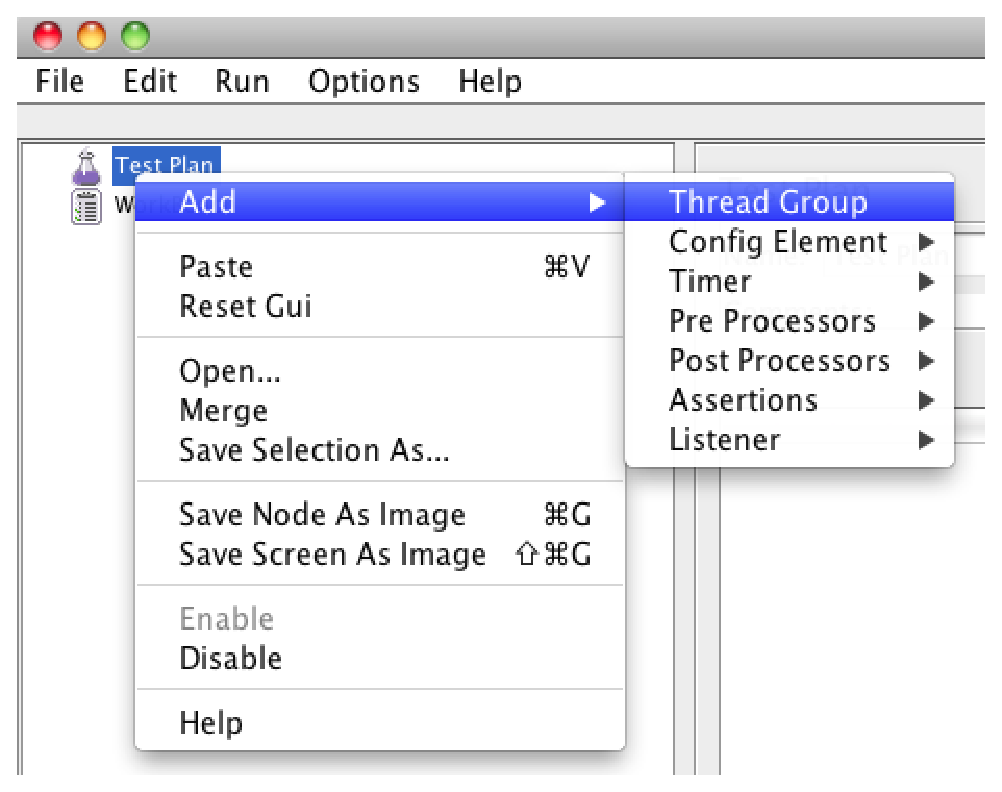
\includegraphics[scale=0.45]{screen/addThreadGroup.eps}	  
  \end{figure}
\end{frame}

\begin{frame}
  \begin{figure}
    \centering
    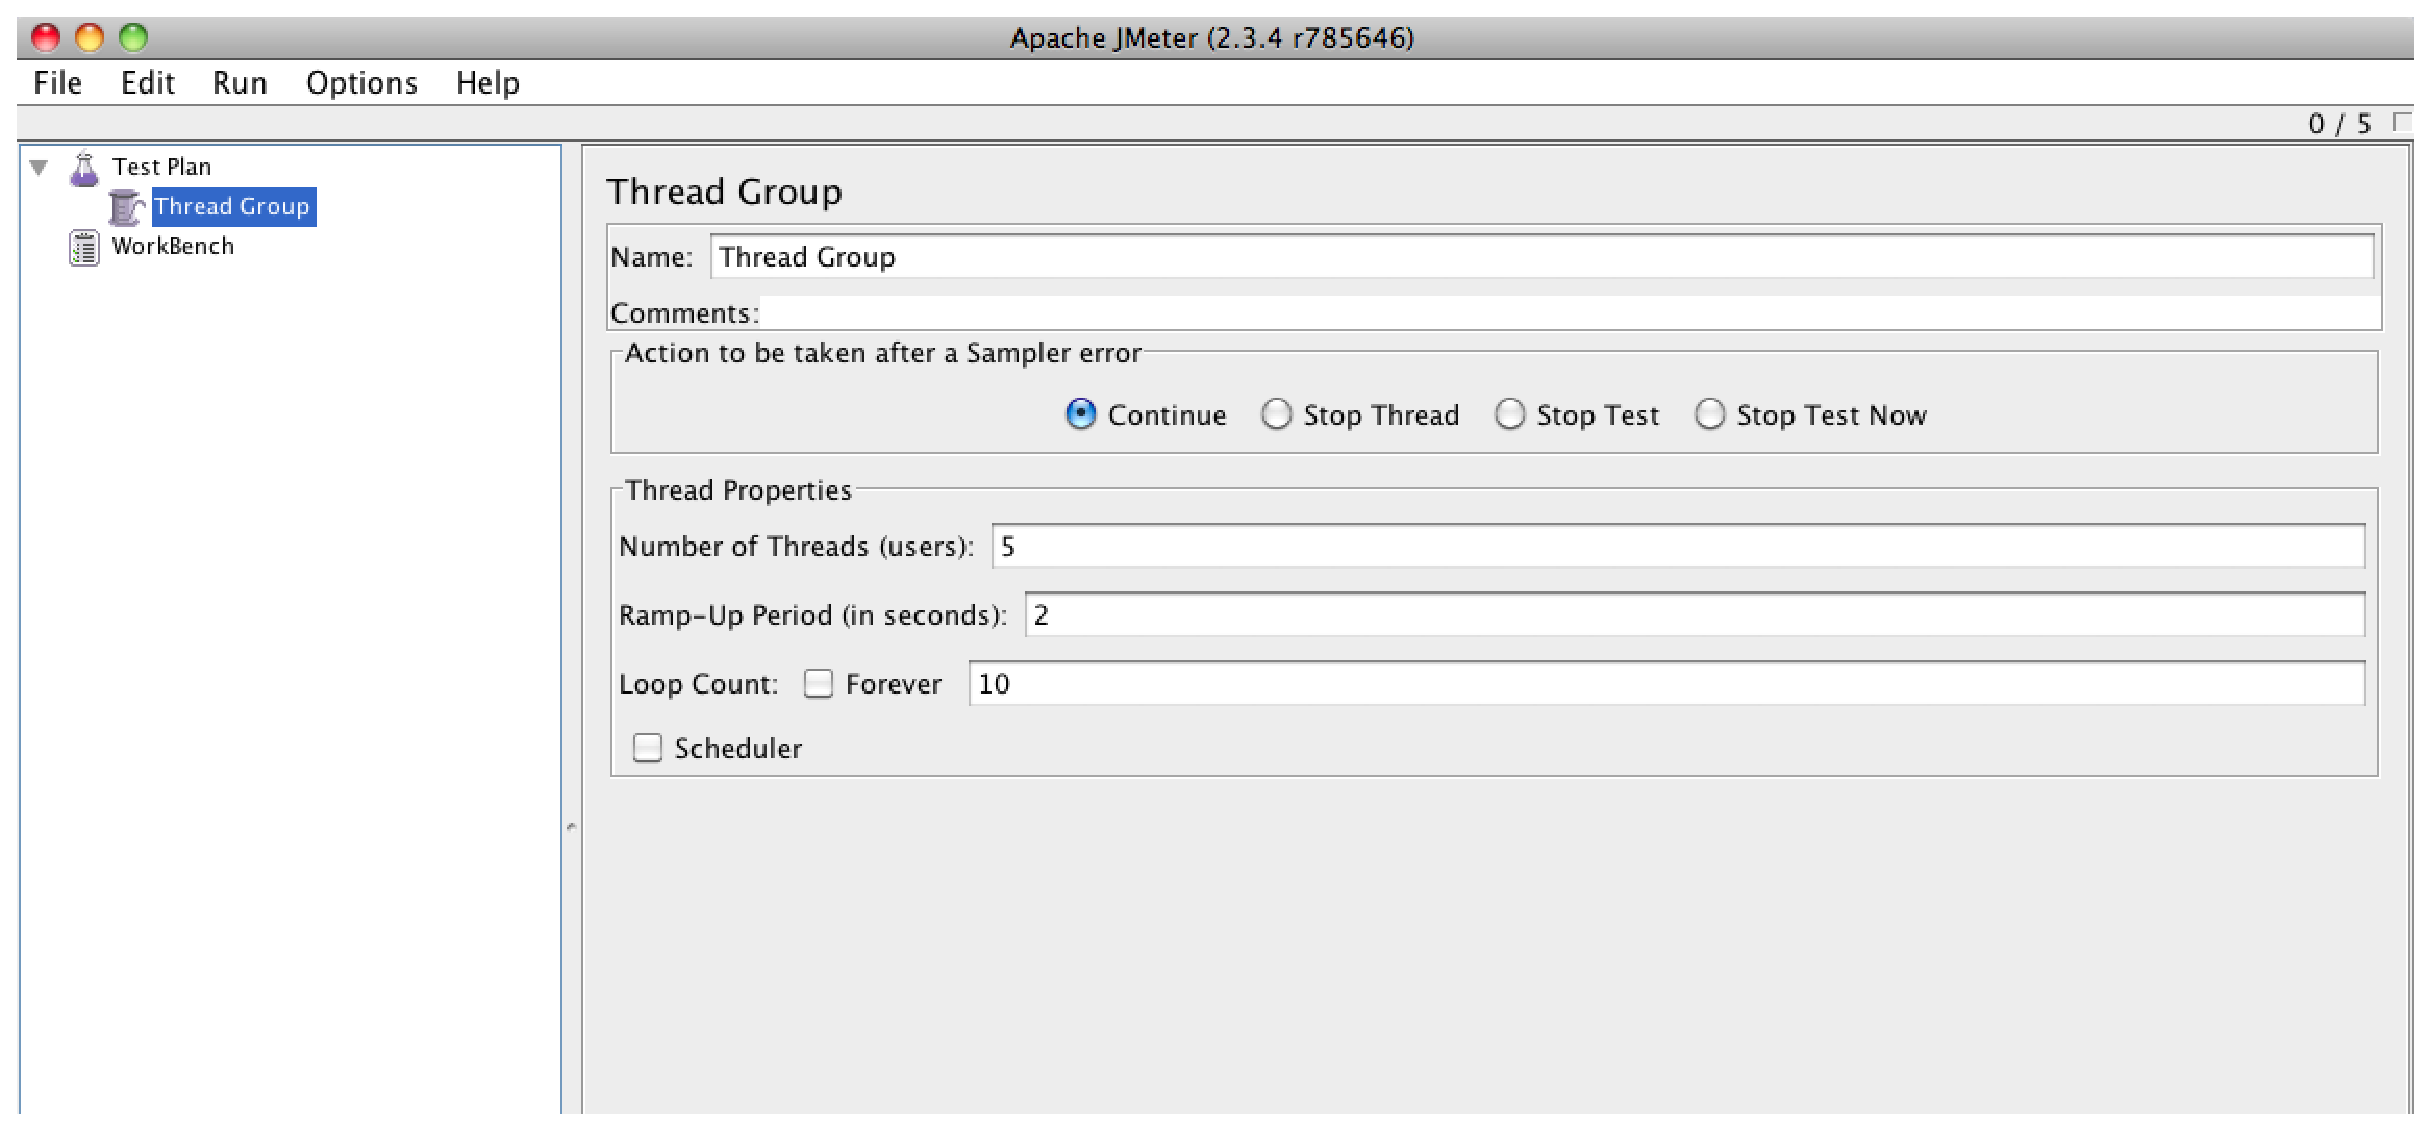
\includegraphics[scale=0.25]{screen/threadGroup.eps}	  
  \end{figure}
\end{frame}

\begin{frame}
  \frametitle{Sampler}
  \begin{itemize}
   \item ``Me�punkt''
   \item Erzeugt Sample Result
    \begin{itemize}
     \item Success?, Request, Response, Headers, Timing, ...
    \end{itemize}
   \item z.B. HTTP Request \bf{HTTPClient}
  \end{itemize}
\end{frame}


\begin{frame}
  \begin{figure}
    \centering
    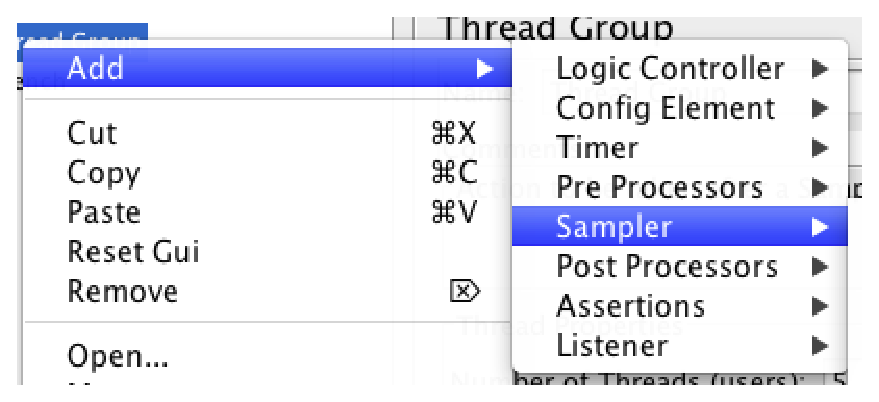
\includegraphics[scale=0.6]{screen/sampler.eps}	  
  \end{figure}
\end{frame}

\begin{frame}
  \begin{figure}
    \centering
    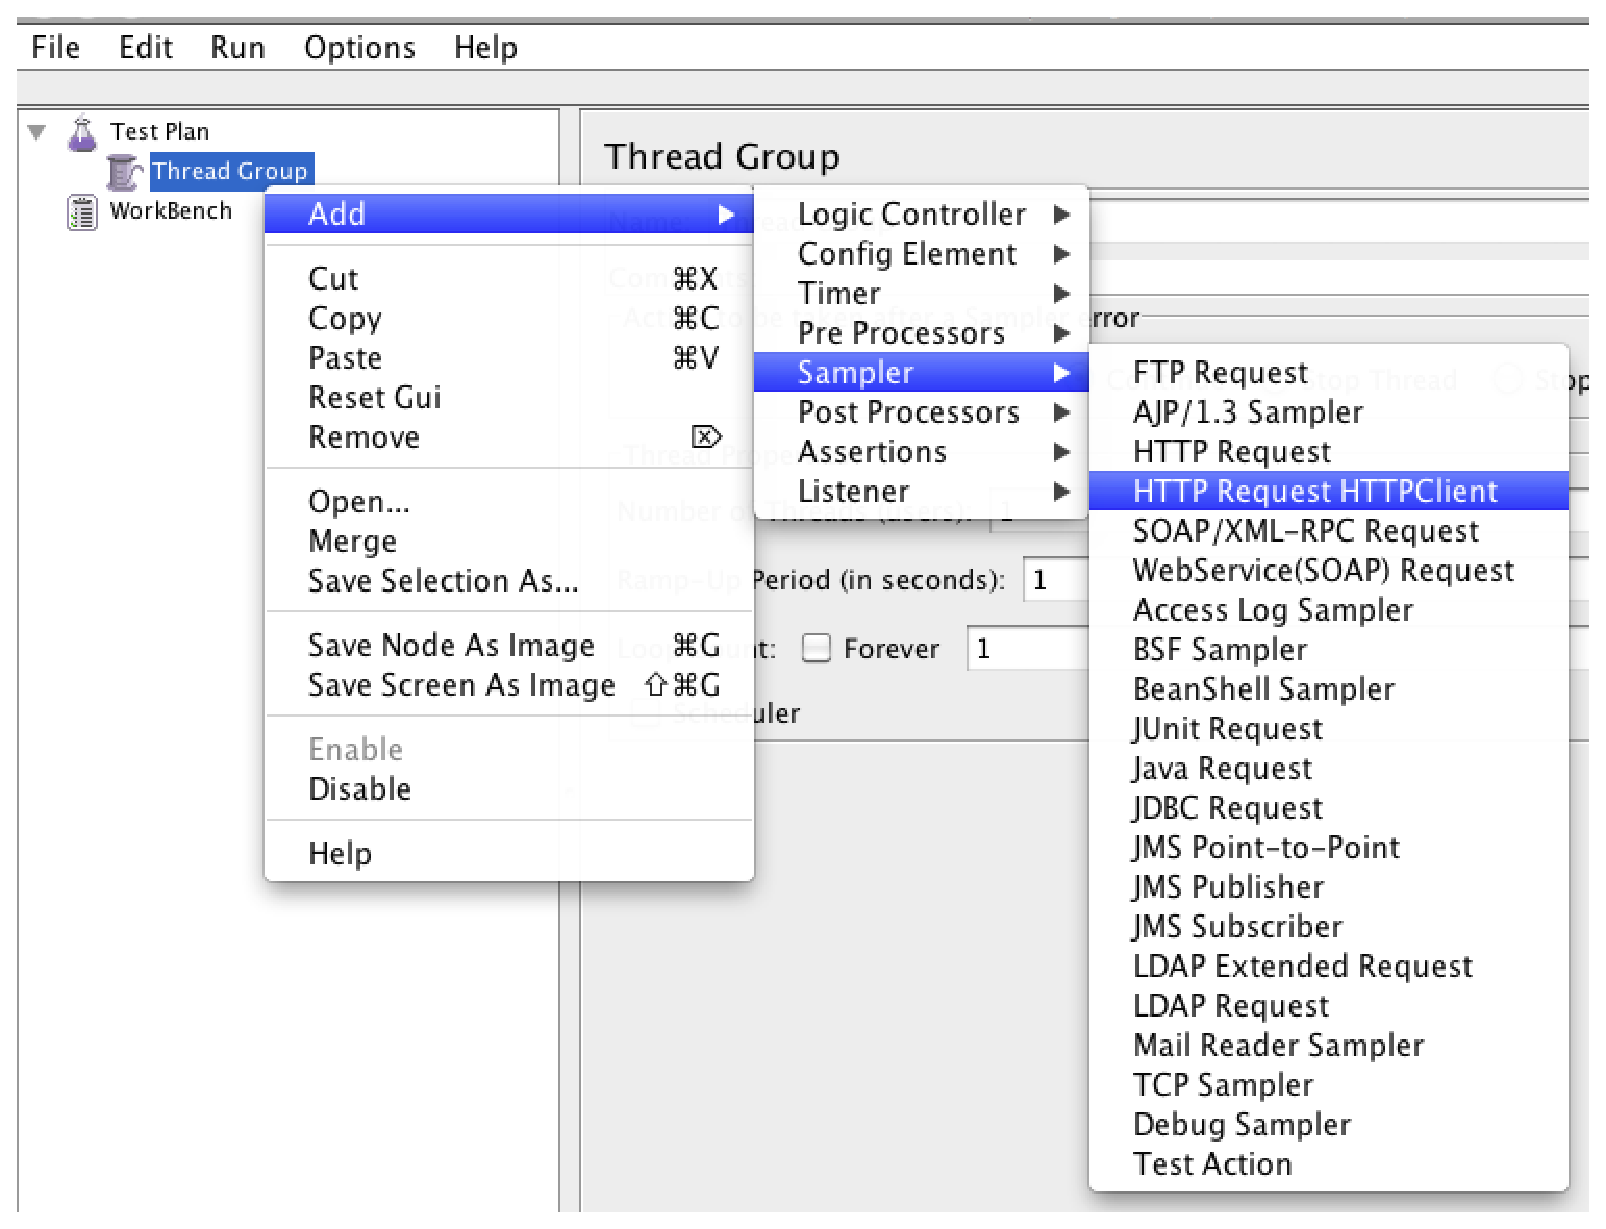
\includegraphics[scale=0.35]{screen/addMenu.eps}	  
  \end{figure}
\end{frame}

\begin{frame}
  \begin{figure}
    \centering
    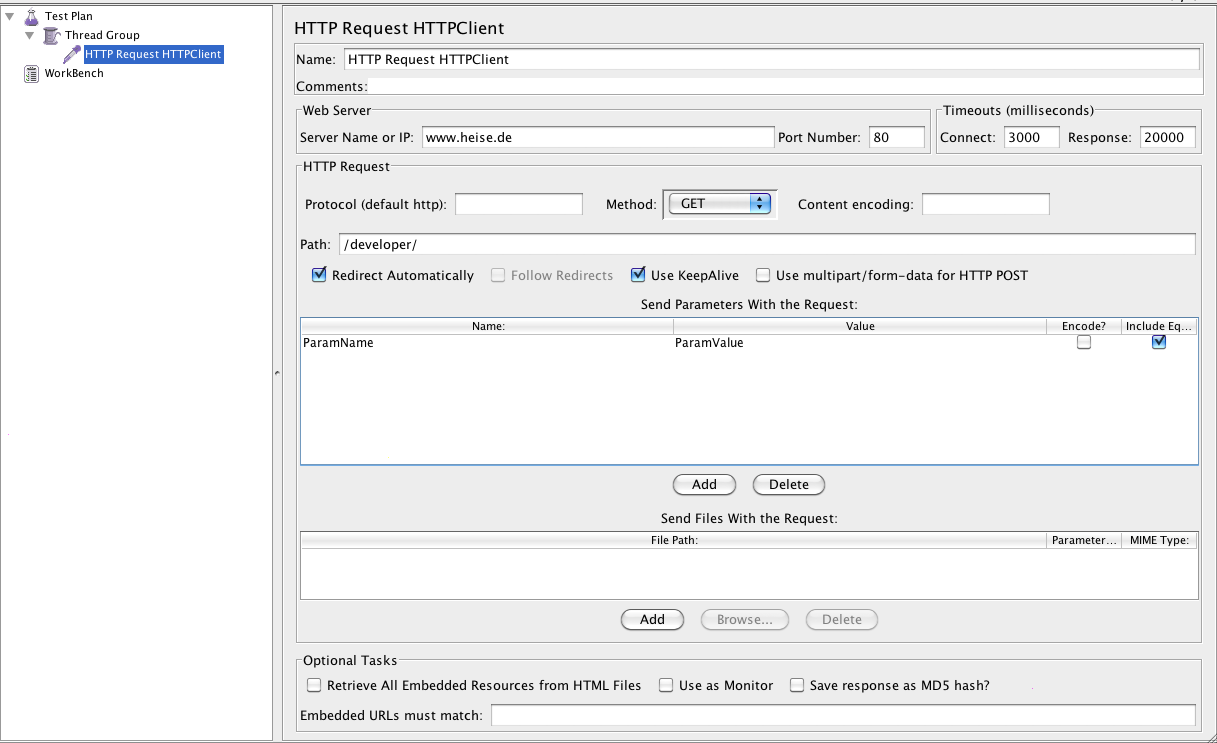
\includegraphics[scale=0.25]{screen/httpSampler.eps}	  
  \end{figure}
\end{frame}

\begin{frame}
  \frametitle{Listener}
  \begin{itemize}
   \item Wertet ein Sample-Result aus
   \item ``View Results Tree'' und ``Summary Report'' sind meine Favoriten
   \item Simple Data Writer (CSV oder XML)
  \end{itemize}
\end{frame}

\begin{frame}
  \begin{figure}
    \centering
    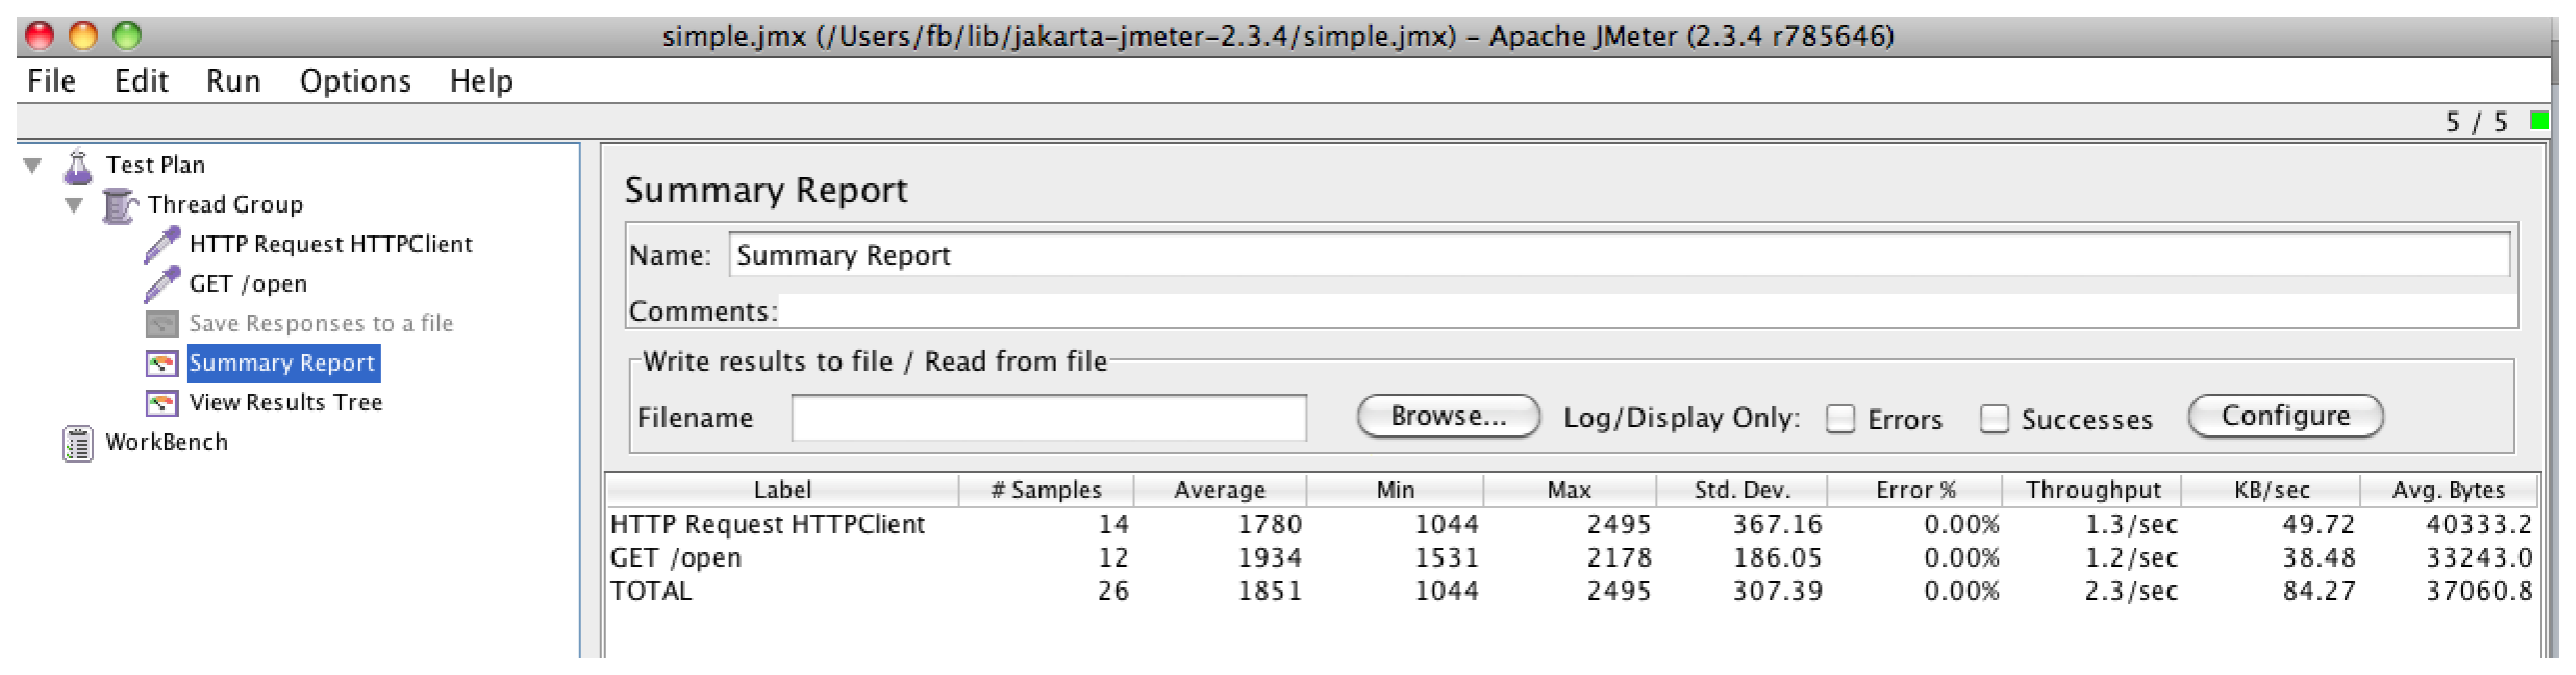
\includegraphics[scale=0.25]{screen/simpleSum.eps}	  
  \end{figure}
\end{frame}

\begin{frame}
  \begin{figure}
    \centering
    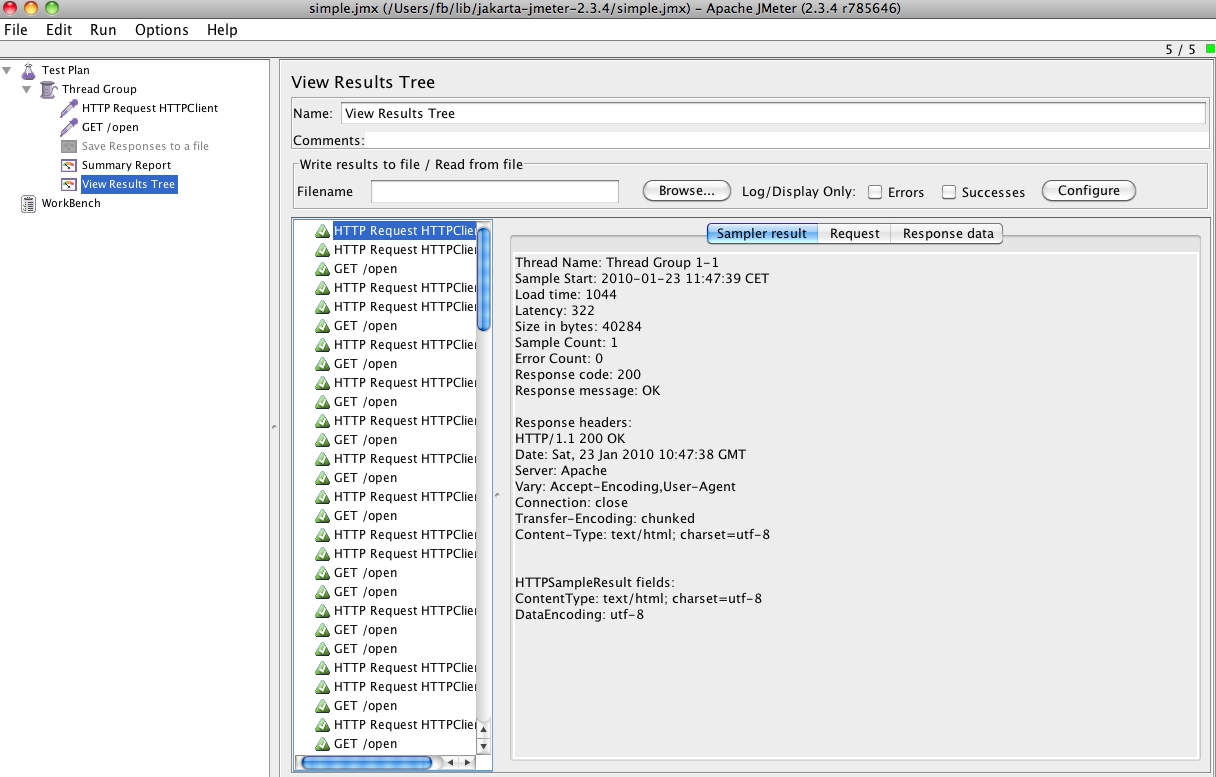
\includegraphics[scale=0.25]{screen/simpleResult.eps}	  
  \end{figure}
\end{frame}

\begin{frame}
  \frametitle{Simpler HTTP-Testplan}
  \begin{figure}
    \centering
    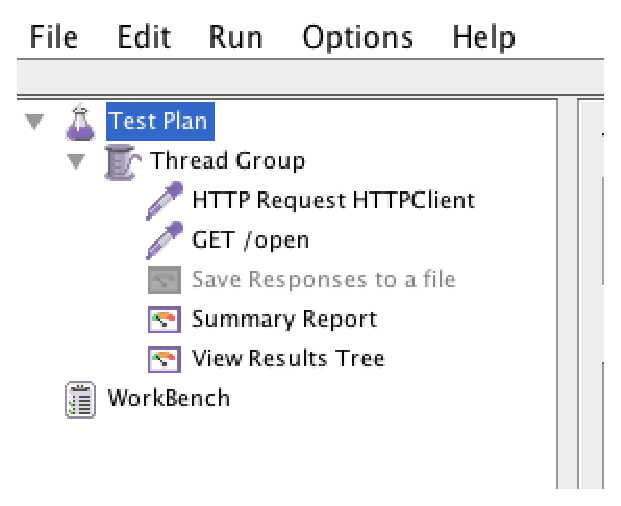
\includegraphics[scale=0.7]{screen/simplePlan.eps}	  
  \end{figure}
\end{frame}


\section{Erweiterungen}
%\begin{frame}
%  \frametitle{Configuration Elements}
%  \begin{itemize}
%   \item Konfigurieren der Sampler etc.
%   \item z.B.: HTTP Request Defaults, Cookie Manager
%  \end{itemize}
%\end{frame}

\begin{frame}
  \frametitle{Assertions}
  \begin{itemize}
   \item analog zu $assert(...)$
   \item Zusicherung wird verletzt $\rightarrow$ Sample fehlgeschlagen
   \item z.B.: Response Assertion, Duration Assertion
  \end{itemize}
\end{frame}

% Demo Simple HTTP Testplan with assert
\begin{frame}
  \begin{figure}
    \centering
    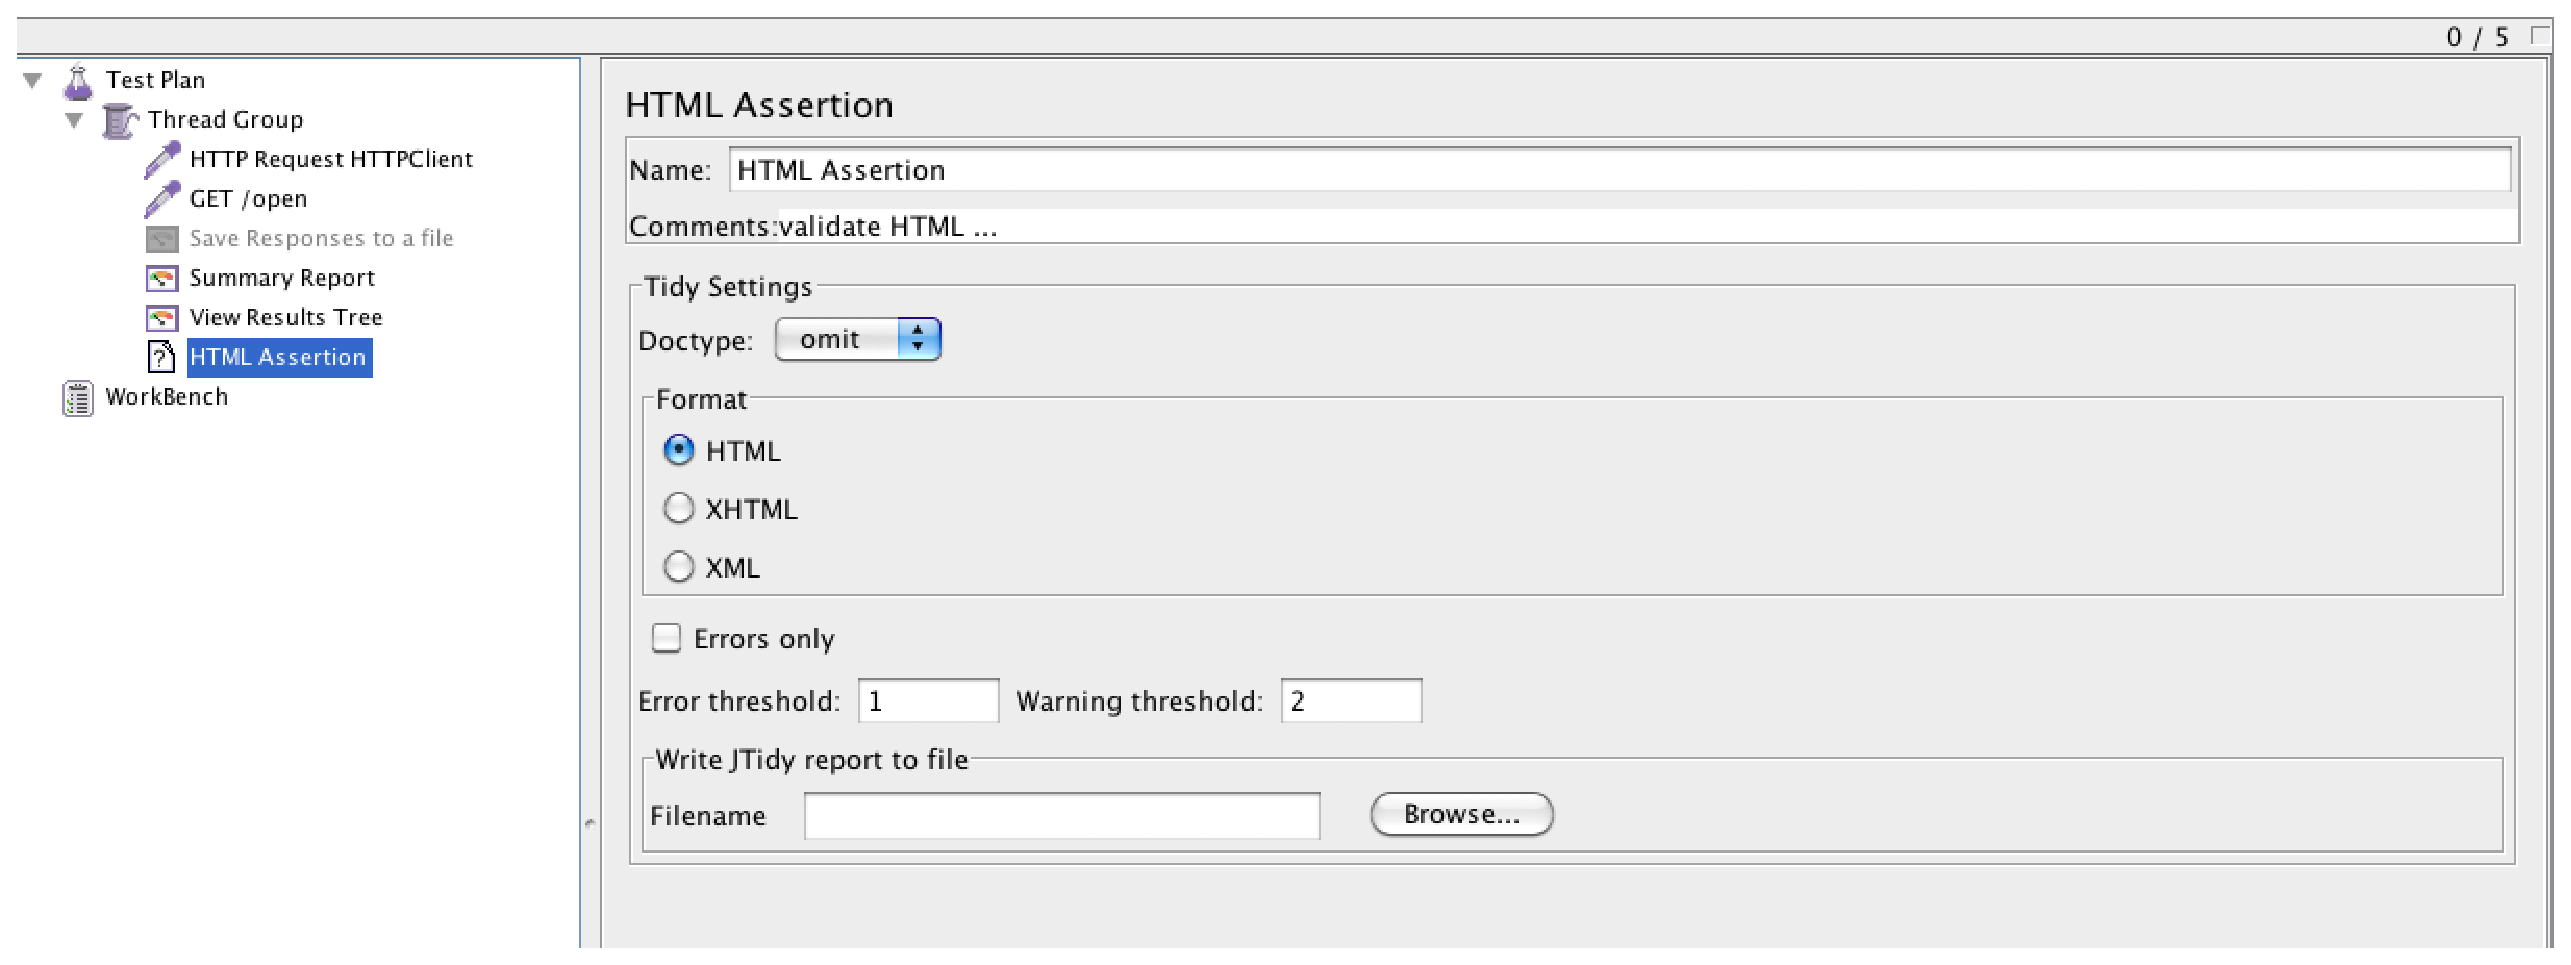
\includegraphics[scale=0.25]{screen/assertHtml.eps}	  
  \end{figure}
\end{frame}

\begin{frame}
  \begin{figure}
    \centering
    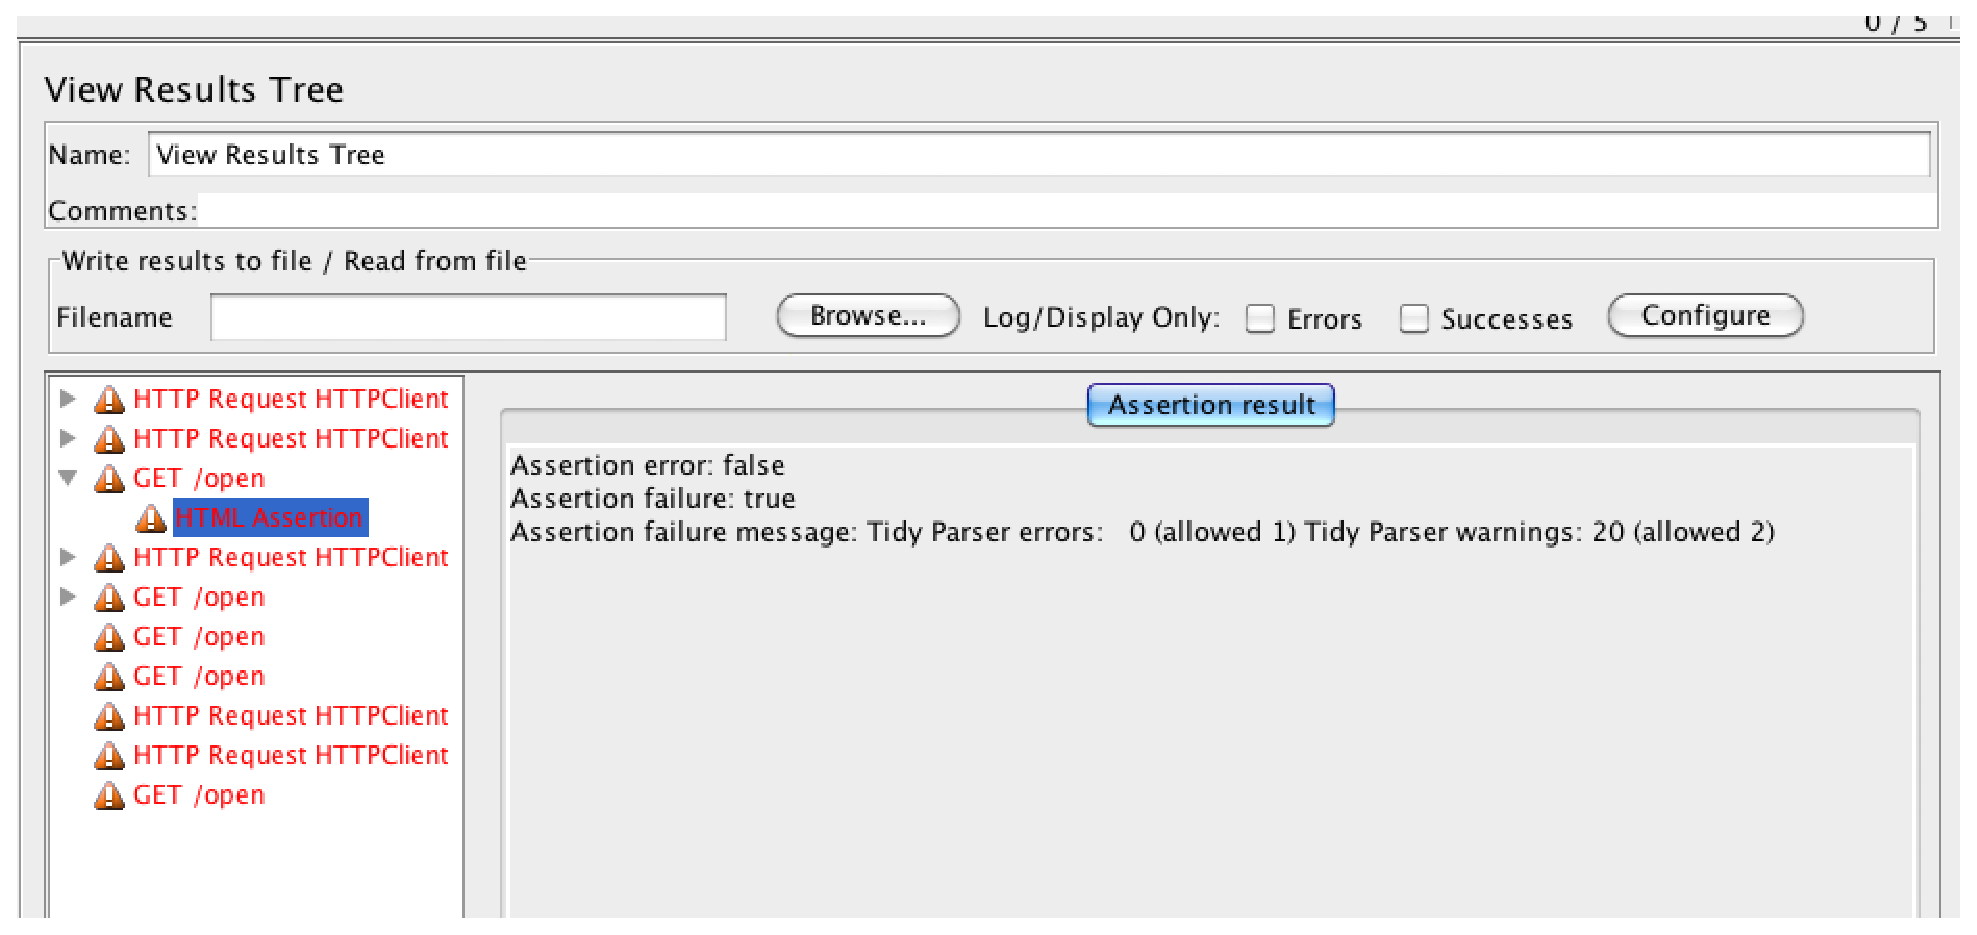
\includegraphics[scale=0.3]{screen/assertResult.eps}	  
  \end{figure}
\end{frame}

\begin{frame}
  \frametitle{Logic Controller}
  \begin{itemize}
   \item �ndern den Kontroll-Flu�
   \item z.B. Loop Controller, Once Only Controller
  \end{itemize}
\end{frame}

% Demo Simple HTTP Testplan with logic and assert
\begin{frame}
  \begin{figure}
    \centering
    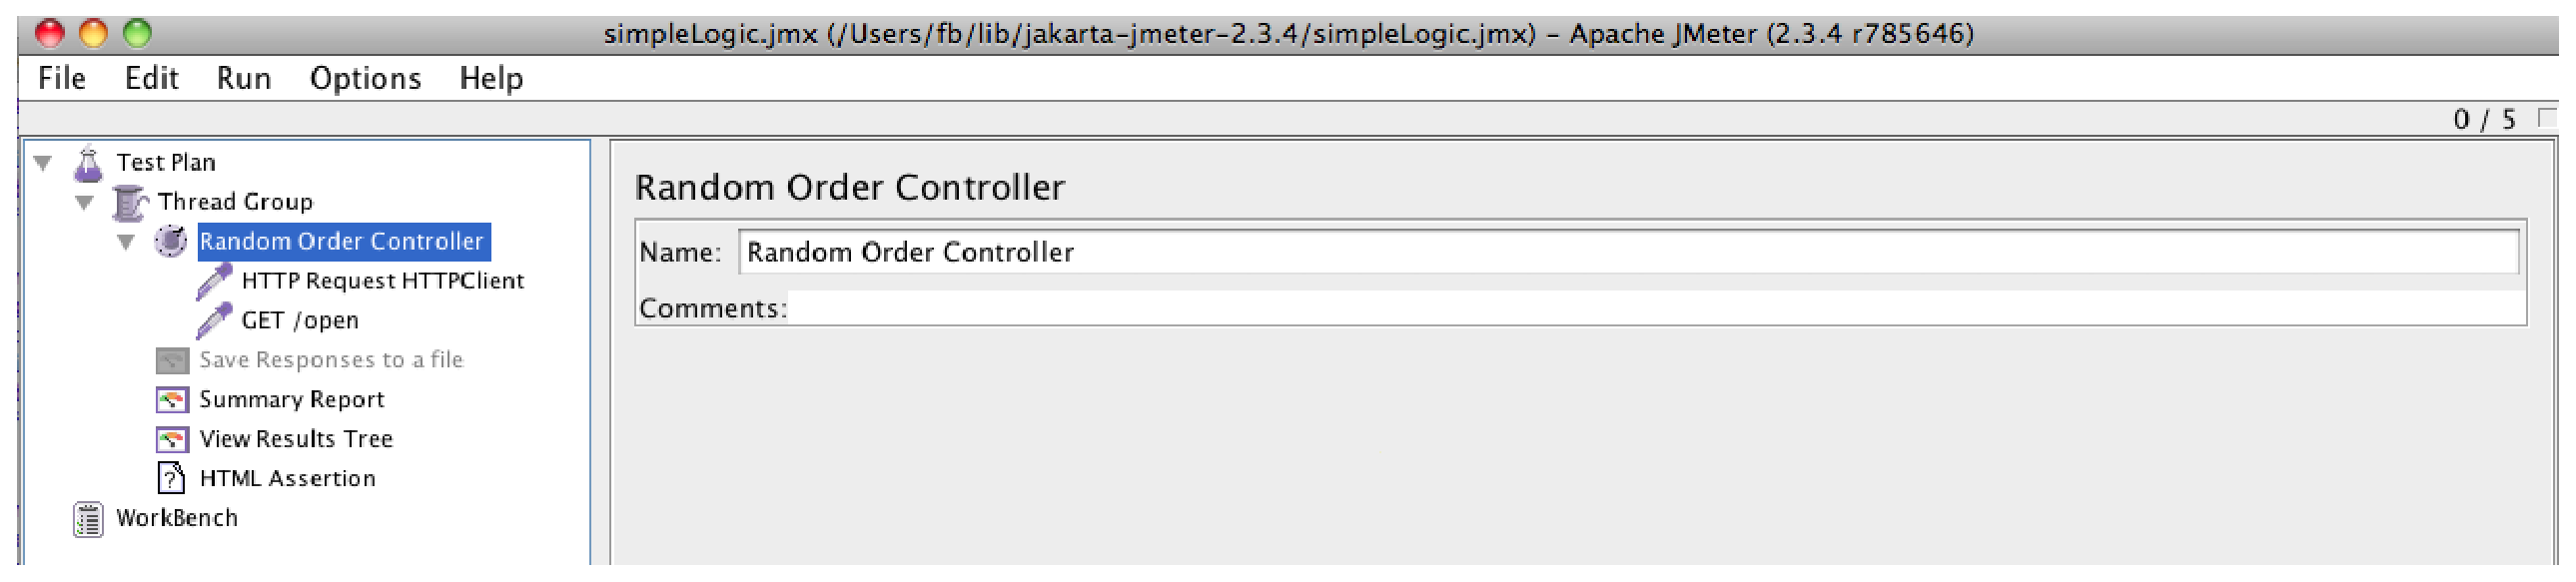
\includegraphics[scale=0.25]{screen/controller.eps}	  
  \end{figure}
\end{frame}

\begin{frame}
  \begin{figure}
    \centering
    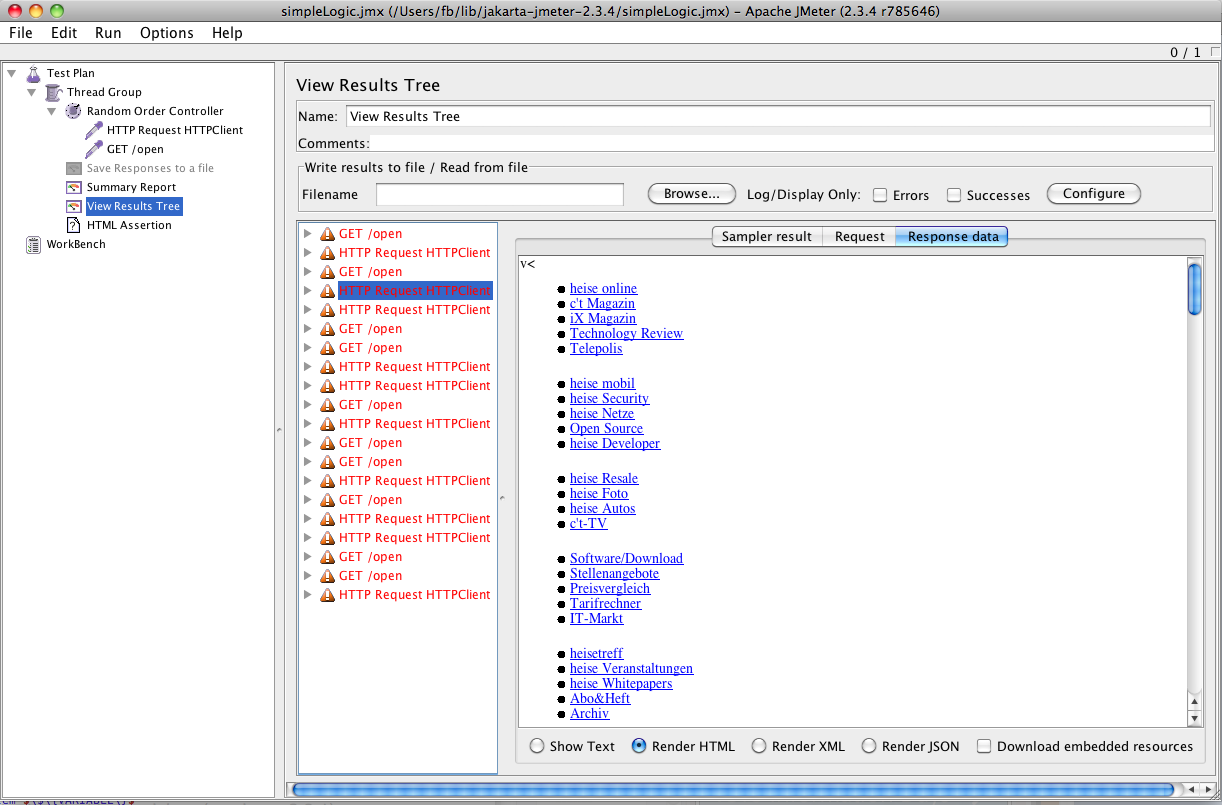
\includegraphics[scale=0.25]{screen/controllerResult.eps}	  
  \end{figure}
\end{frame}

\begin{frame}
\bf{\center{Fragen?}}
\end{frame}

\section{Testpl�ne parametrisieren}
\begin{frame}
  \frametitle{Variablen}
  \begin{itemize}
   \item $\$\{VARIABLE\}$
   \item $\$\{UNDEF\} == UNDEF$
   \item JMeter trim()ed Leerzeichen (Version > 2.3.1)
  \end{itemize}
\end{frame}

\begin{frame}
  \frametitle{Funktionen}
  \begin{itemize}
   \item $\$\{\_\_functionName(var1,var2,var3)\}$
   \item $\$\{\_\_threadNum\}$
   \item $\$\{\_\_Random(1,63,LOTTERY)\}$
   \item $\$\{\_\_javaScript(expr,RETVAL)\}$
   \item Escape ``,'' as ``\textbackslash,''
  \end{itemize}
\end{frame}

\begin{frame}
  \frametitle{Funktionen}
  \begin{figure}
    \centering
    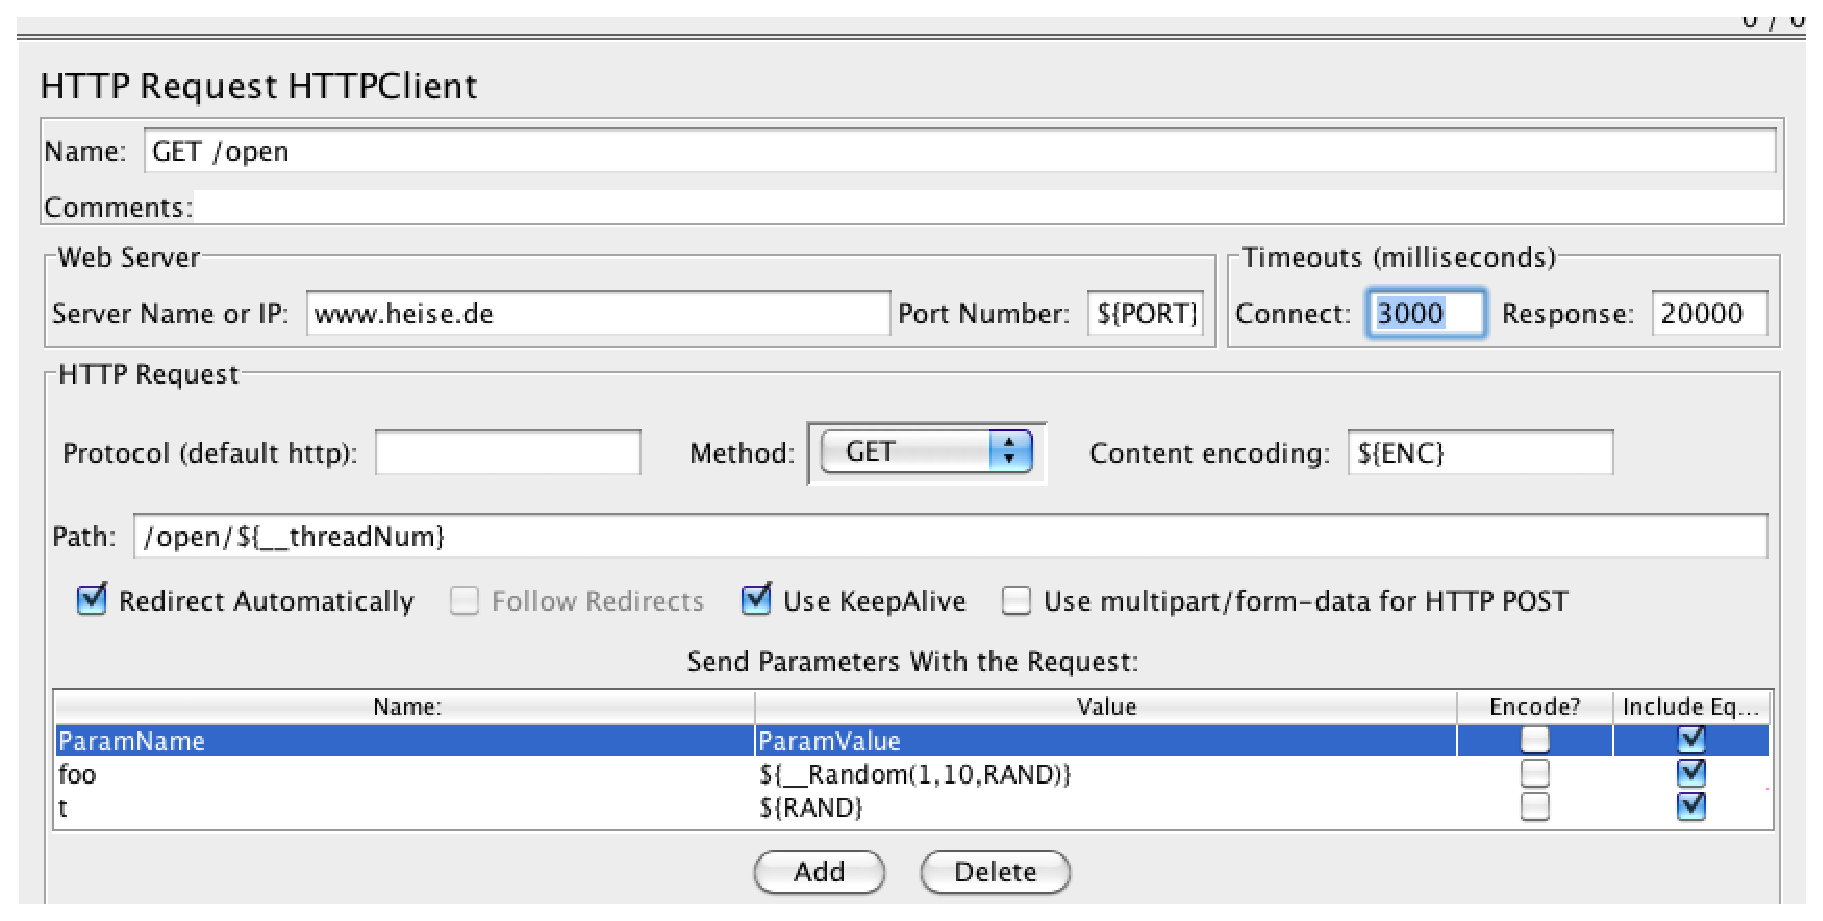
\includegraphics[scale=0.35]{screen/random.eps}	  
  \end{figure}
\end{frame}

%\begin{frame}
%  \frametitle{Testplan File-Format}
%  \begin{itemize}
%   \item JMX (JMeter XML)
%   \item Fast selbsterkl�rend ($cat\ \$plan$)
%   \item Kann man gut mit sed, xslt, ruby etc. erzeugen ... \pause
%   \item ... und mit maven ausf�hren
%  \end{itemize}
%\end{frame}

%\begin{frame}
%  \frametitle{Interessante Sampler}
%  \begin{itemize}
%   \item JUnit3 Sampler / JUnit4 Sampler
%   \item Access Log Sampler
%   \begin{itemize}
%    \item Leider keine POST-Parameter
%   \end{itemize}
%   \item SOAP Sampler
%  \end{itemize}
%\end{frame}


\section{Fallstricke}

\begin{frame}
  \frametitle{Fallstricke}
  \begin{itemize}
   \item Synchrones I/O, $n \geq 1000$ Threads
   \item Einige Sampler machen ineffizentes I/O (z.B. DNS)
   \item HTTP Request \uline{HTTPClient} vs. \sout{HTTP Request}
   \item Java GC (500ms Full GC $ \rightarrow $ Test steht 0,5sec)
  \end{itemize}
\end{frame}

\begin{frame}
  \frametitle{Fallstricke}
  \begin{itemize}
   \item WhileController eval()ed eine JMeter-Funktion\pause
   \item IfController eval()ed JavaScript
   \begin{itemize}
     \item Jedes JavaScript-Statements muss mit ``;'' enden\pause
   \end{itemize}
   \item ``Read the fine source (and fix it)''
   \item Parametrisierung von Testpl�nen ist etwas anstrengend
  \end{itemize}
\end{frame}

\begin{frame}
  \frametitle{Fehlersuche}
  \begin{itemize}
   \item View Result in Tree (evtl. mit ``log errors only'')
   \item Test mit einen Thread und einen Loop-Count von eins laufen lassen
   \item JMeter-Log-Level in \texttt{bin/jmeter.properties} erh�hen
   \item ``What's this node?'' Men�-Option gibt Klassennamen aus
   \item Live HTTP Headers und Firebug Firefox-Plugins
  \end{itemize}
\end{frame}

\begin{frame}
  \frametitle{Live HTTP Headers}
  \begin{figure}
    \centering
    \includegraphics[scale=0.2]{screen/liveGen.eps}	  
  \end{figure}
\end{frame}


\begin{frame}
  \begin{figure}
    \centering
    \includegraphics[scale=0.25]{screen/liveHeaders.eps}	  
  \end{figure}
\end{frame}

\begin{frame}
  \begin{figure}
    \centering
    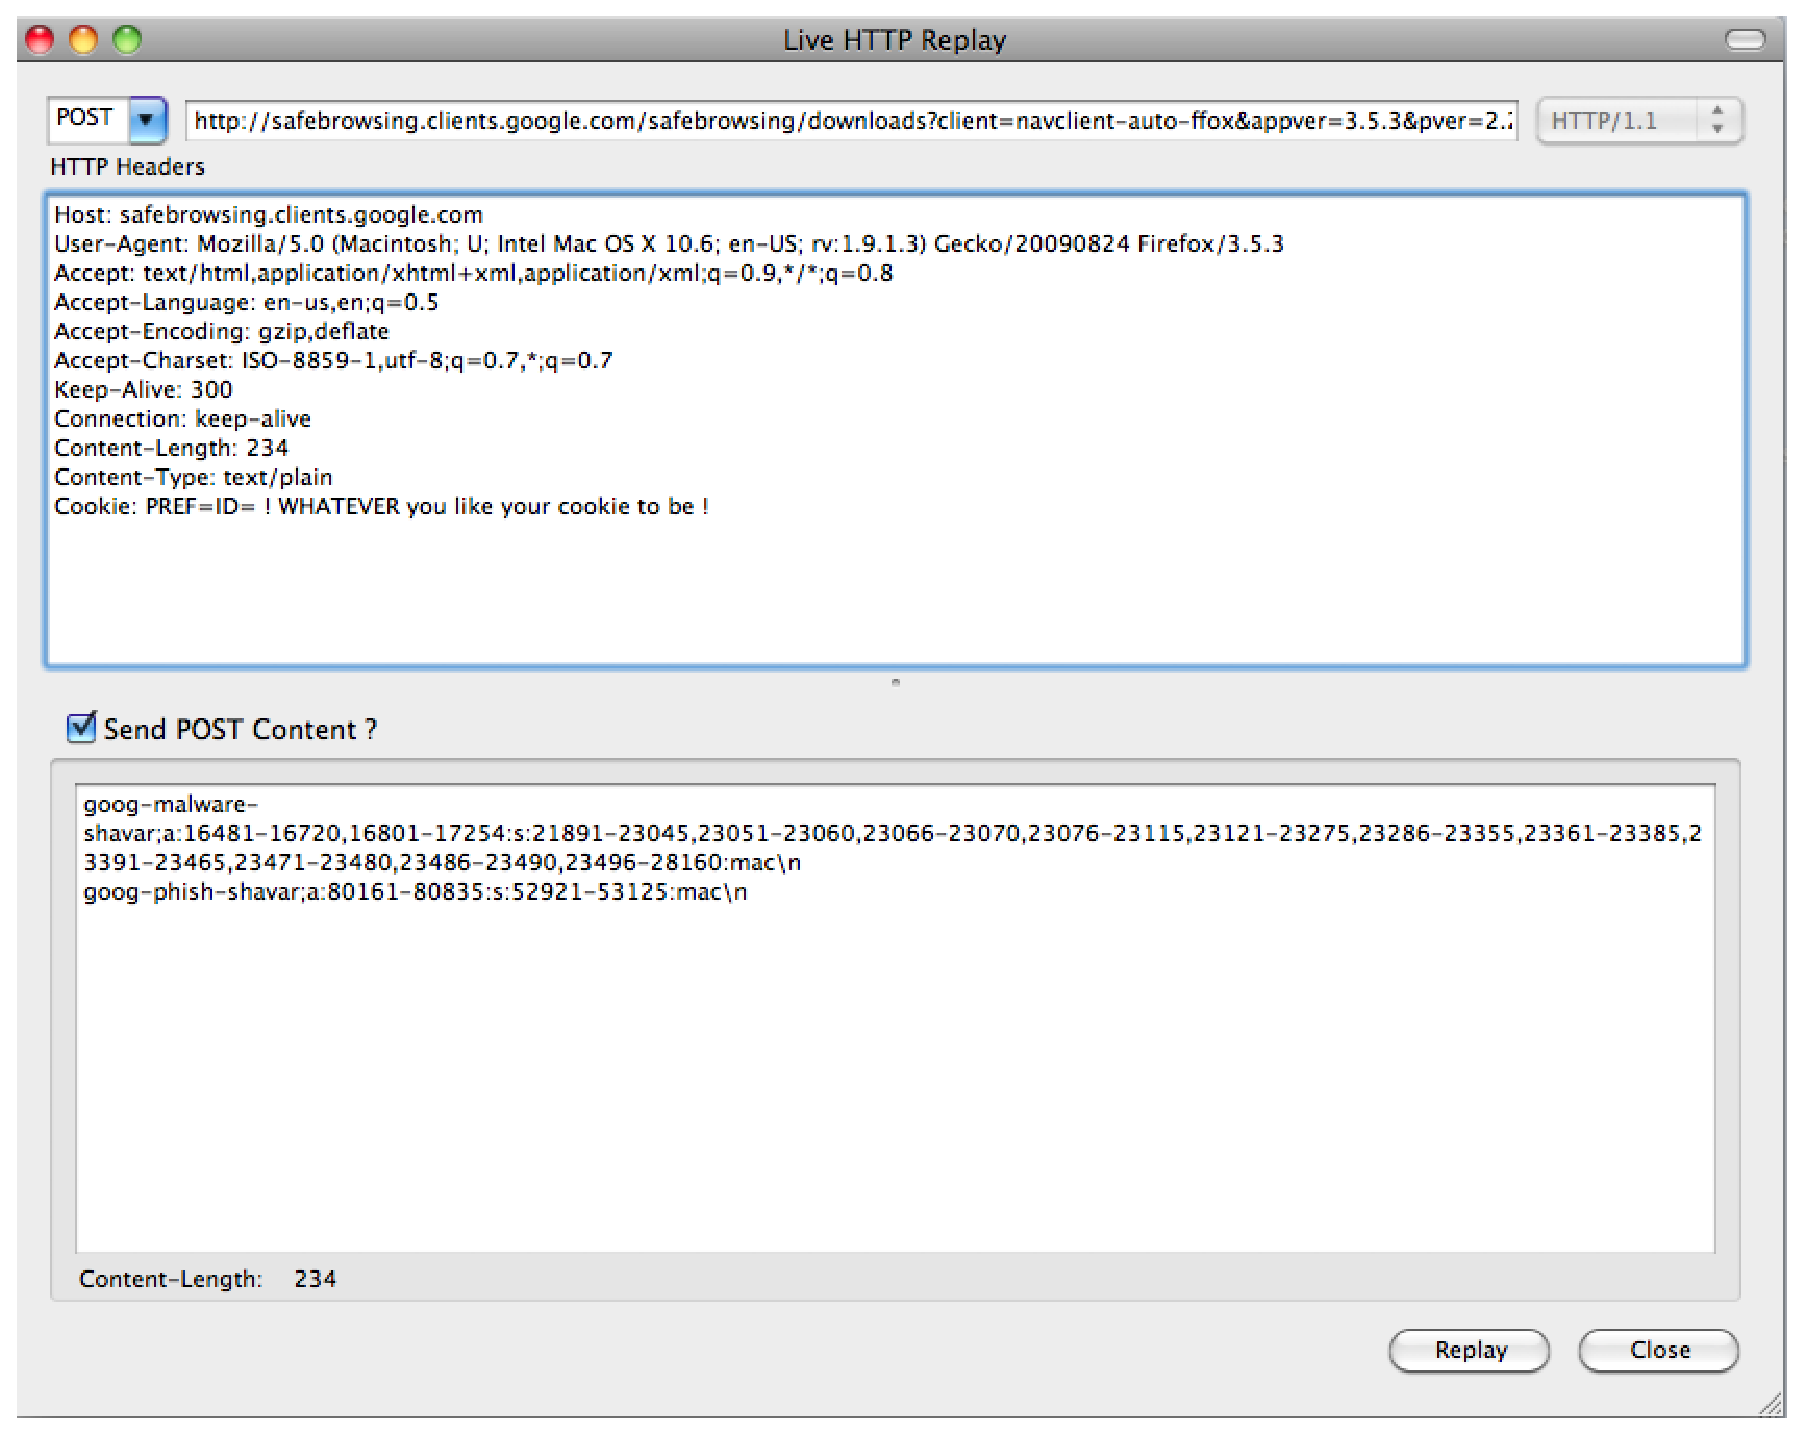
\includegraphics[scale=0.3]{screen/liveReplay.eps}	  
  \end{figure}
\end{frame}

\section{Zusammenfassung}

\begin{frame}
  \frametitle{Zusammenfassung}
  \begin{itemize}
   \item Konzepte
   \item Testpl�ne und Parametrisierung 
   \item Fallstricke 
  \end{itemize}
\end{frame}

\begin{frame}
  \frametitle{Dokumentation}
  \begin{small}
  \begin{itemize}
   \item \url{http://jakarta.apache.org/jmeter/usermanual/}
   \item ``Help! My boss wants me to load test our web app!''
   \begin{itemize}
     \begin{scriptsize}
       \item \url{http://jakarta.apache.org/jmeter/usermanual/boss.html}
     \end{scriptsize}
   \end{itemize}
   \item Mailinglisten 
   \begin{itemize}
     \begin{scriptsize}
       \item \url{http://jakarta.apache.org/site/mail2.html\#JMeter}
     \end{scriptsize}
    \end{itemize}
   \item \texttt{svn co \url{http://svn.apache.org/repos/asf/jakarta/jmeter/}}
  \end{itemize}
  \end{small}
\end{frame}


\begin{frame}
\center{\bf{Danke!}}
\end{frame}

\begin{frame}
\center{\bf{Fragen? Anregungen? Kritik?}}
\end{frame}

%\begin{frame}
%\center{\bf{Danke f�r Eure Aufmerksamkeit!}}
%\end{frame}


%\section{Fillers}

\begin{frame}
  \frametitle{Access Log Testplan}
  \begin{figure}
    \centering
    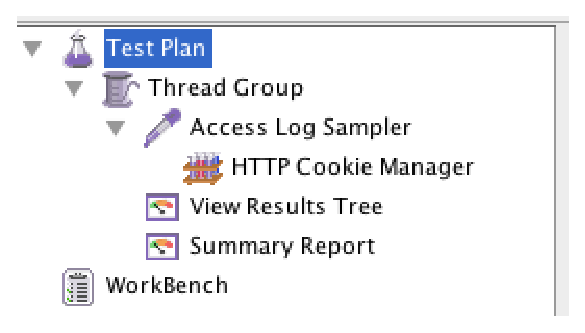
\includegraphics[scale=0.7]{screen/accessLog-Plan.eps}	  
  \end{figure}
\end{frame}


\begin{frame}
  \frametitle{Access Log Sampler}
  \begin{figure}
    \centering
    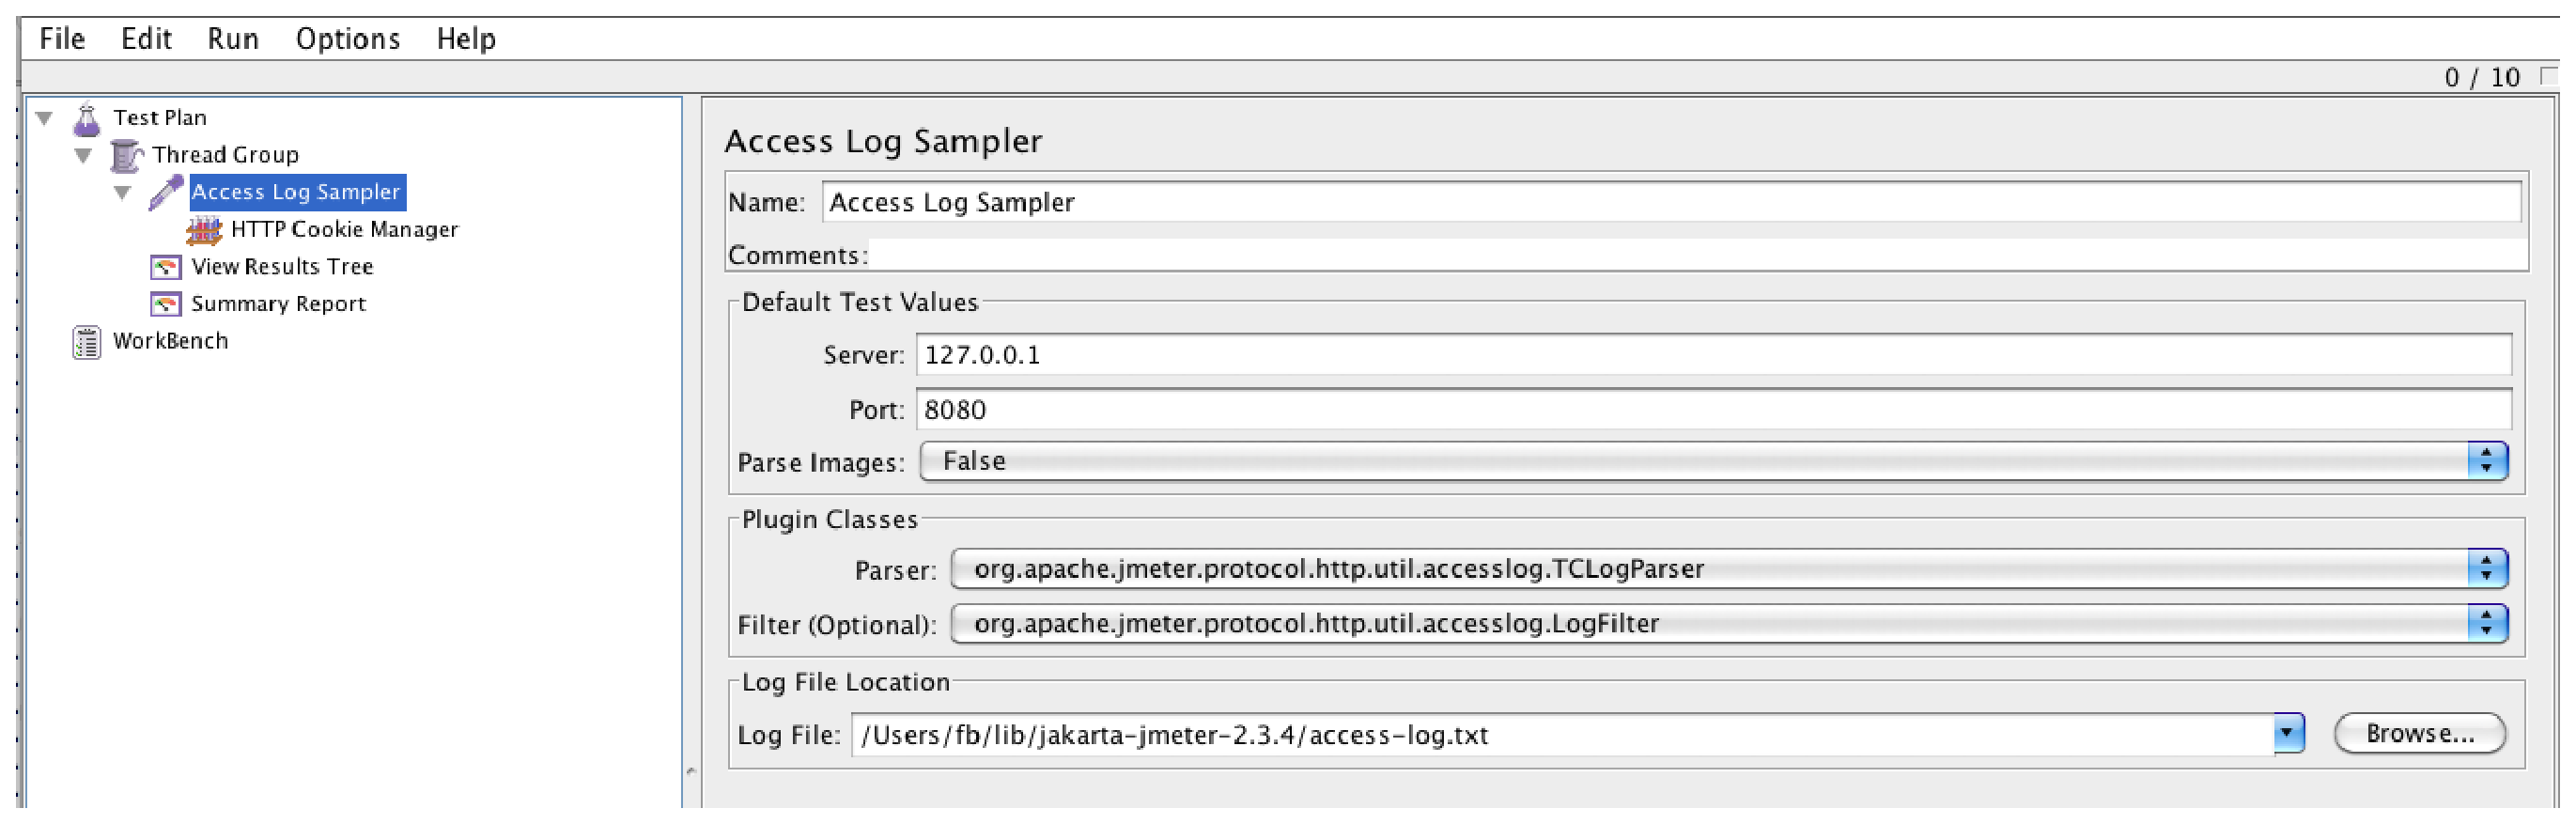
\includegraphics[scale=0.23]{screen/accessLog.eps}	  
   %\caption{Access Log Sampler}
  \end{figure}
\end{frame}

\begin{frame}
  \frametitle{Access Log Sampler}
  \begin{itemize}
    \item Keine POST-Parameter
    \item Session Filter
    \item Cookie Manager sorgt f�r die richtigen\texttrademark \ Cookies
  \end{itemize}
\end{frame}

\begin{frame}
  \begin{figure}
    \centering
    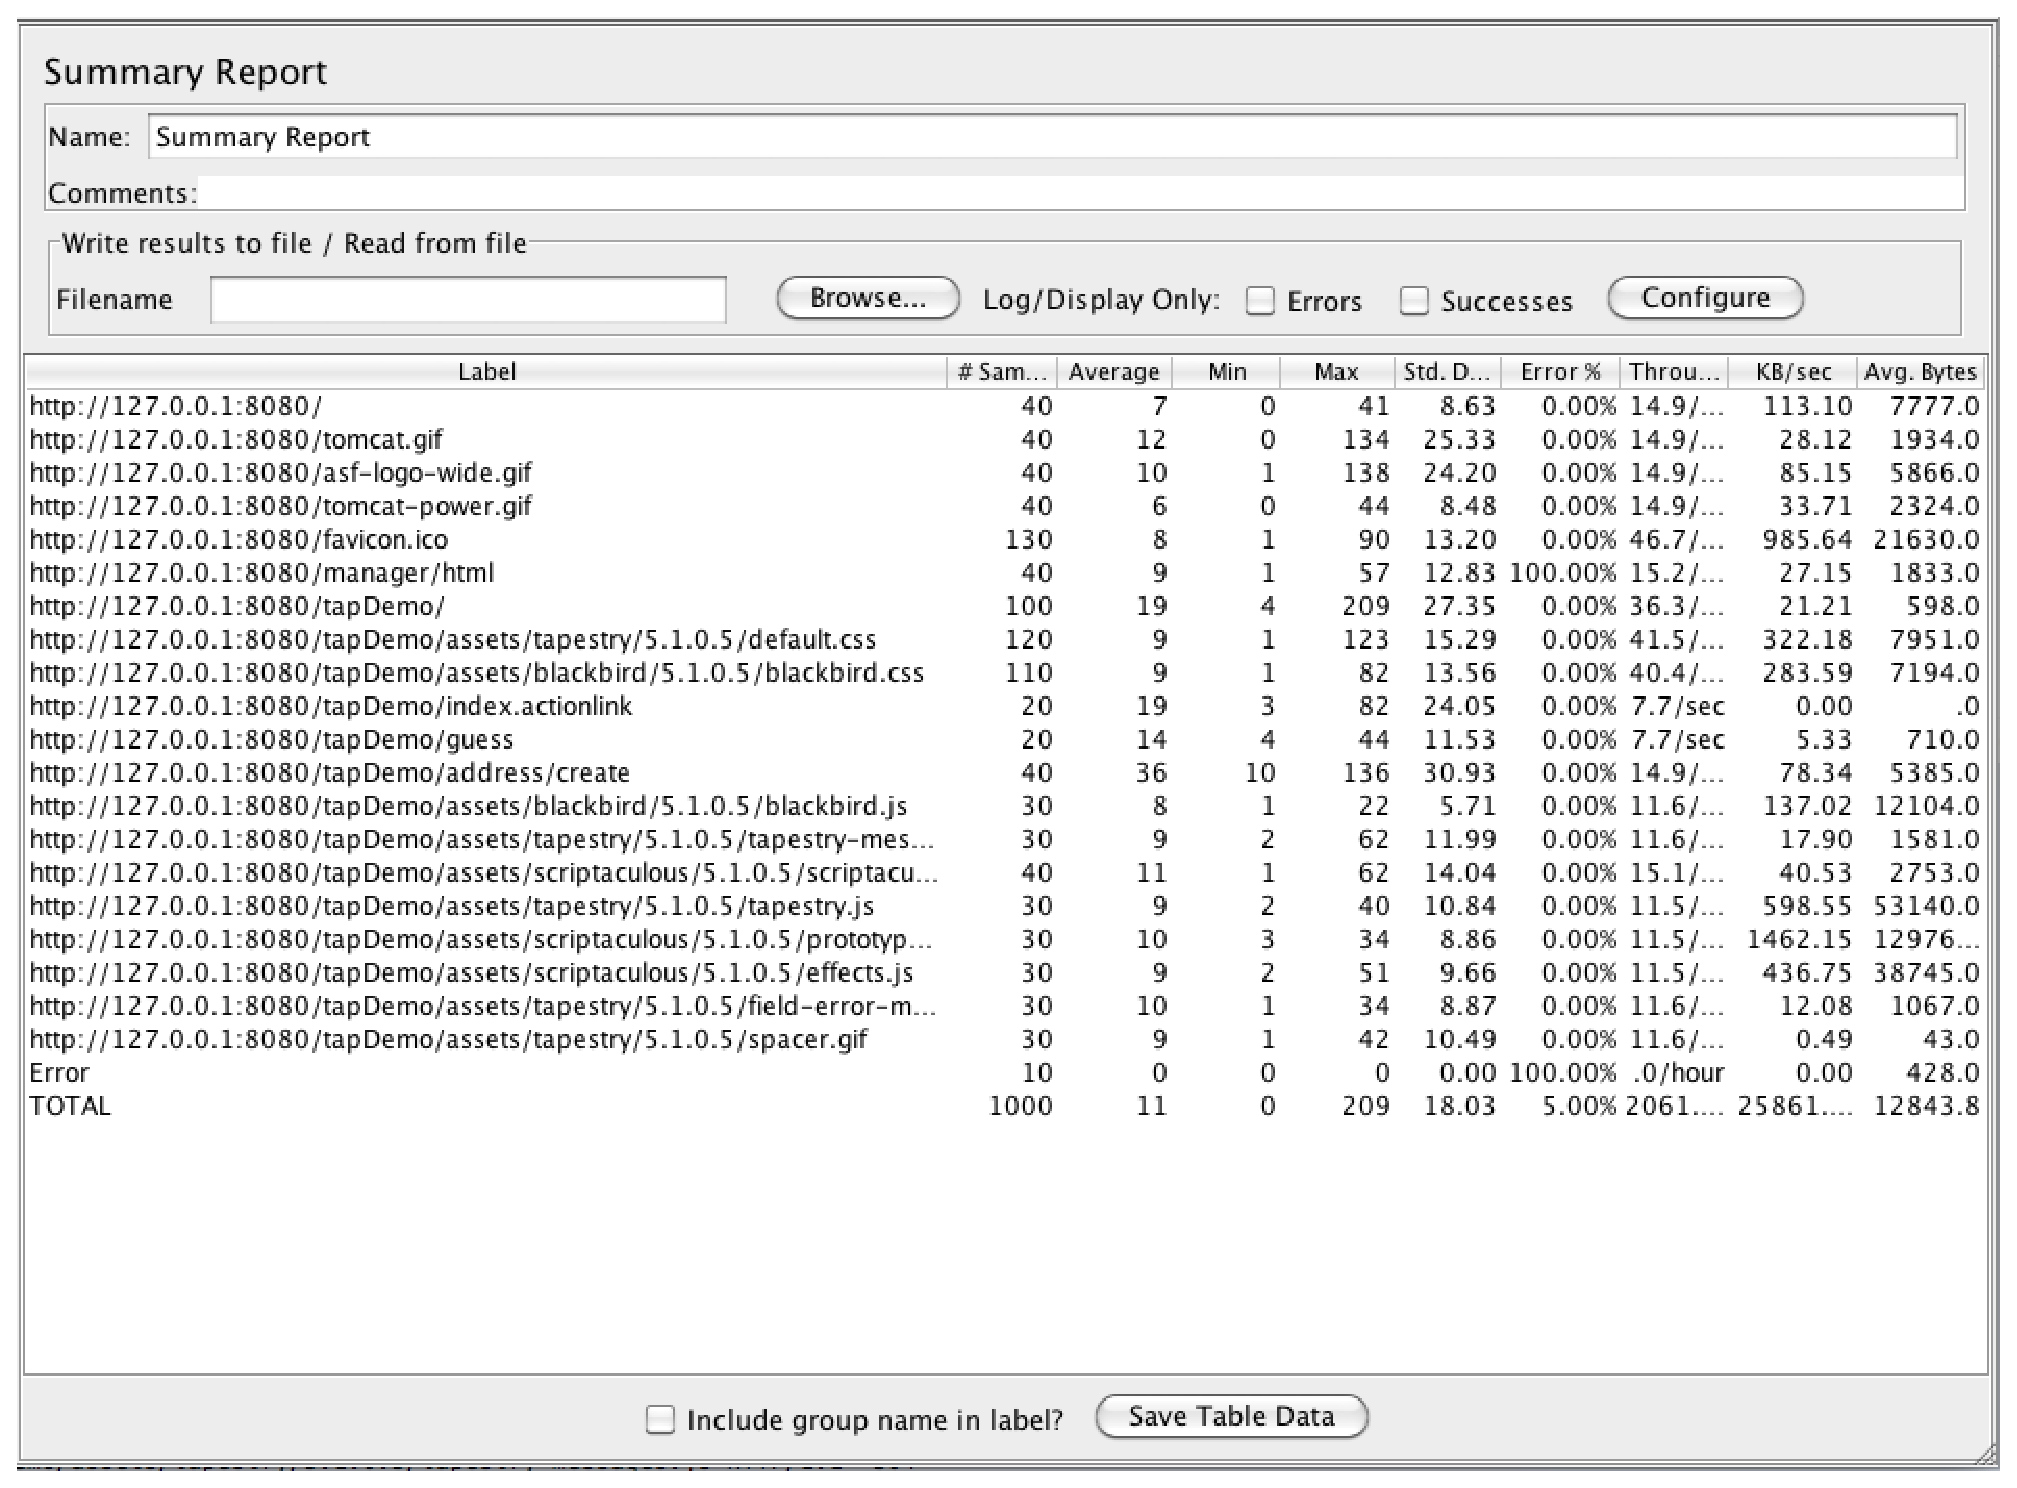
\includegraphics[scale=0.3]{screen/accessLog-Summary.eps}	  
  \end{figure}
\end{frame}

\begin{frame}
  \frametitle{Sample Result}
  \begin{figure}
    \centering
    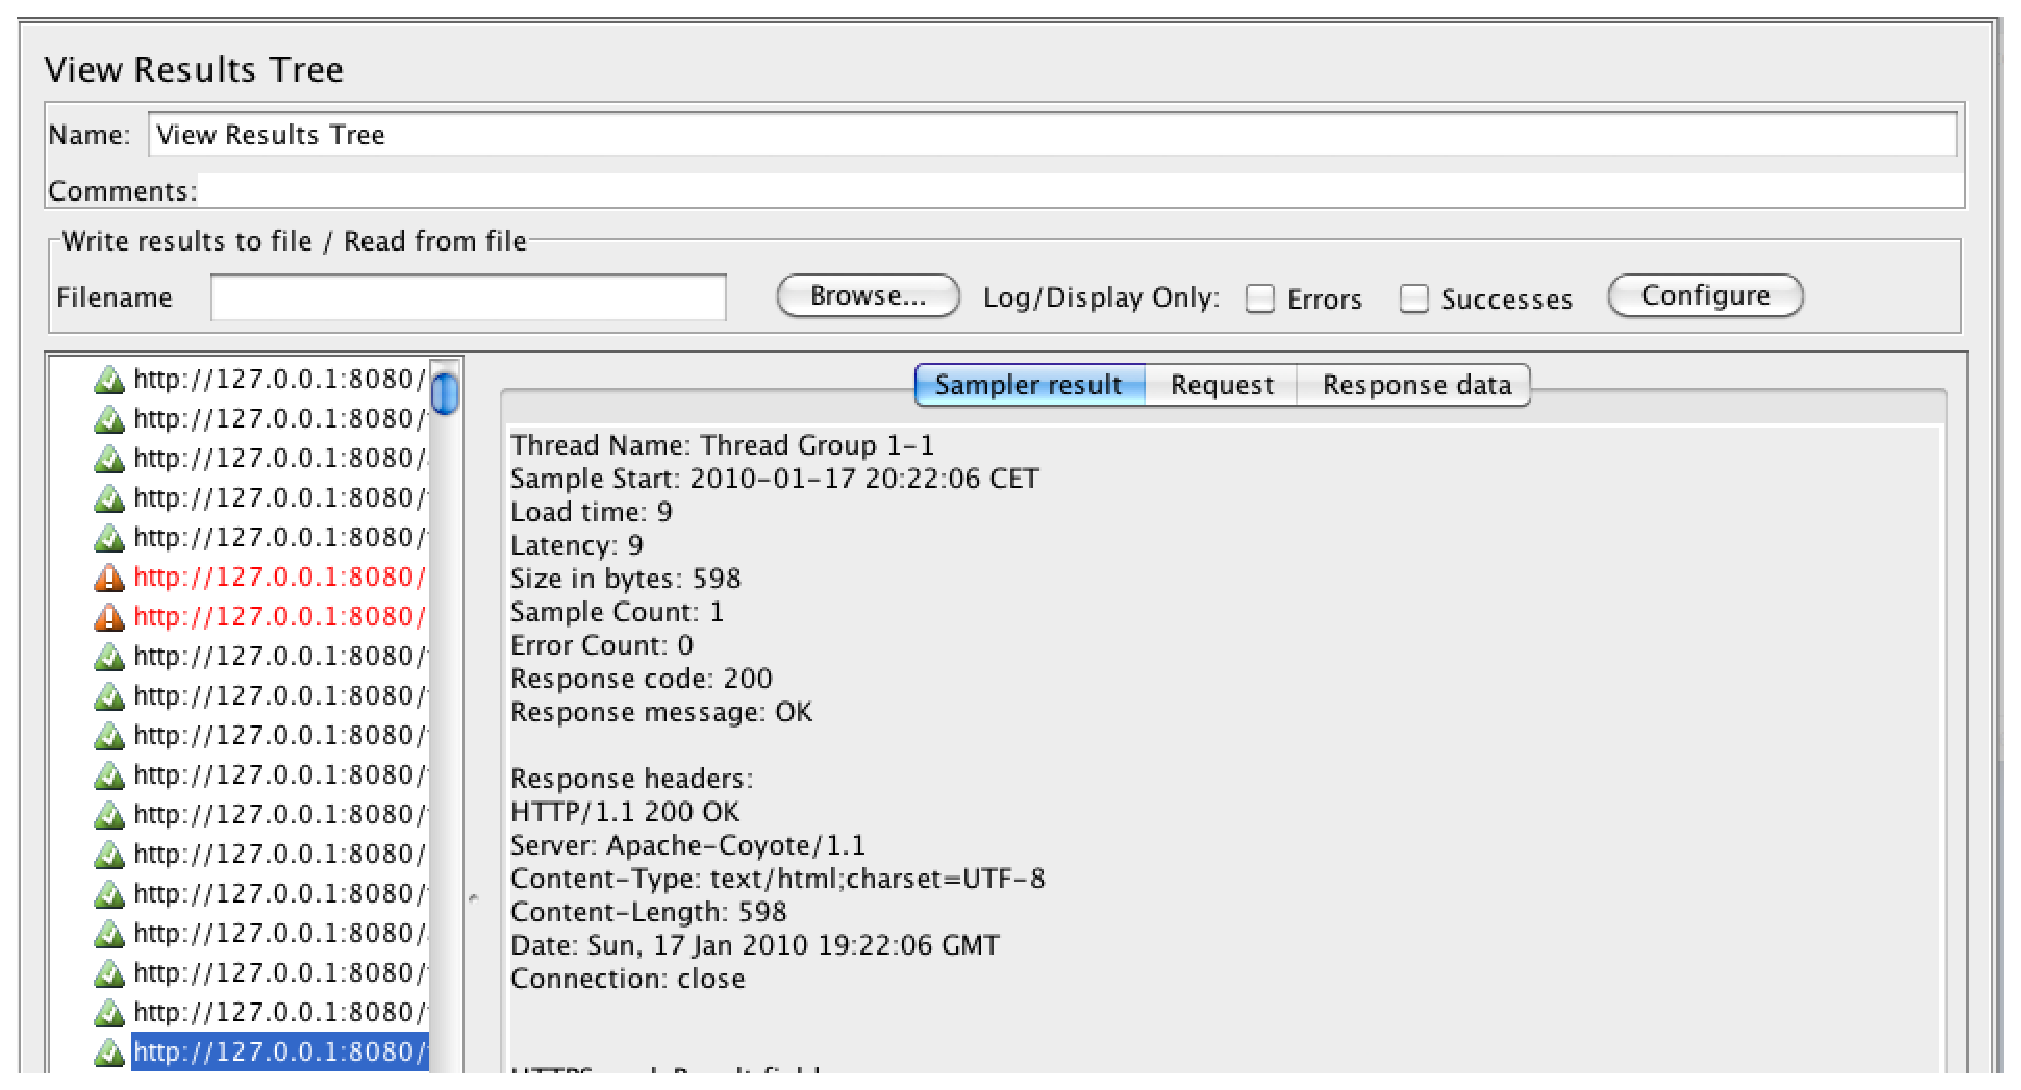
\includegraphics[scale=0.3]{screen/resultTree-Result.eps}	  
  \end{figure}
\end{frame}

\begin{frame}
  \frametitle{Sample Request}
  \begin{figure}
    \centering
    \includegraphics[scale=0.25]{screen/accessLog-ResultTree.eps}	  
  \end{figure}
\end{frame}

\begin{frame}
  \frametitle{Sample Response}
  \begin{figure}
    \centering
    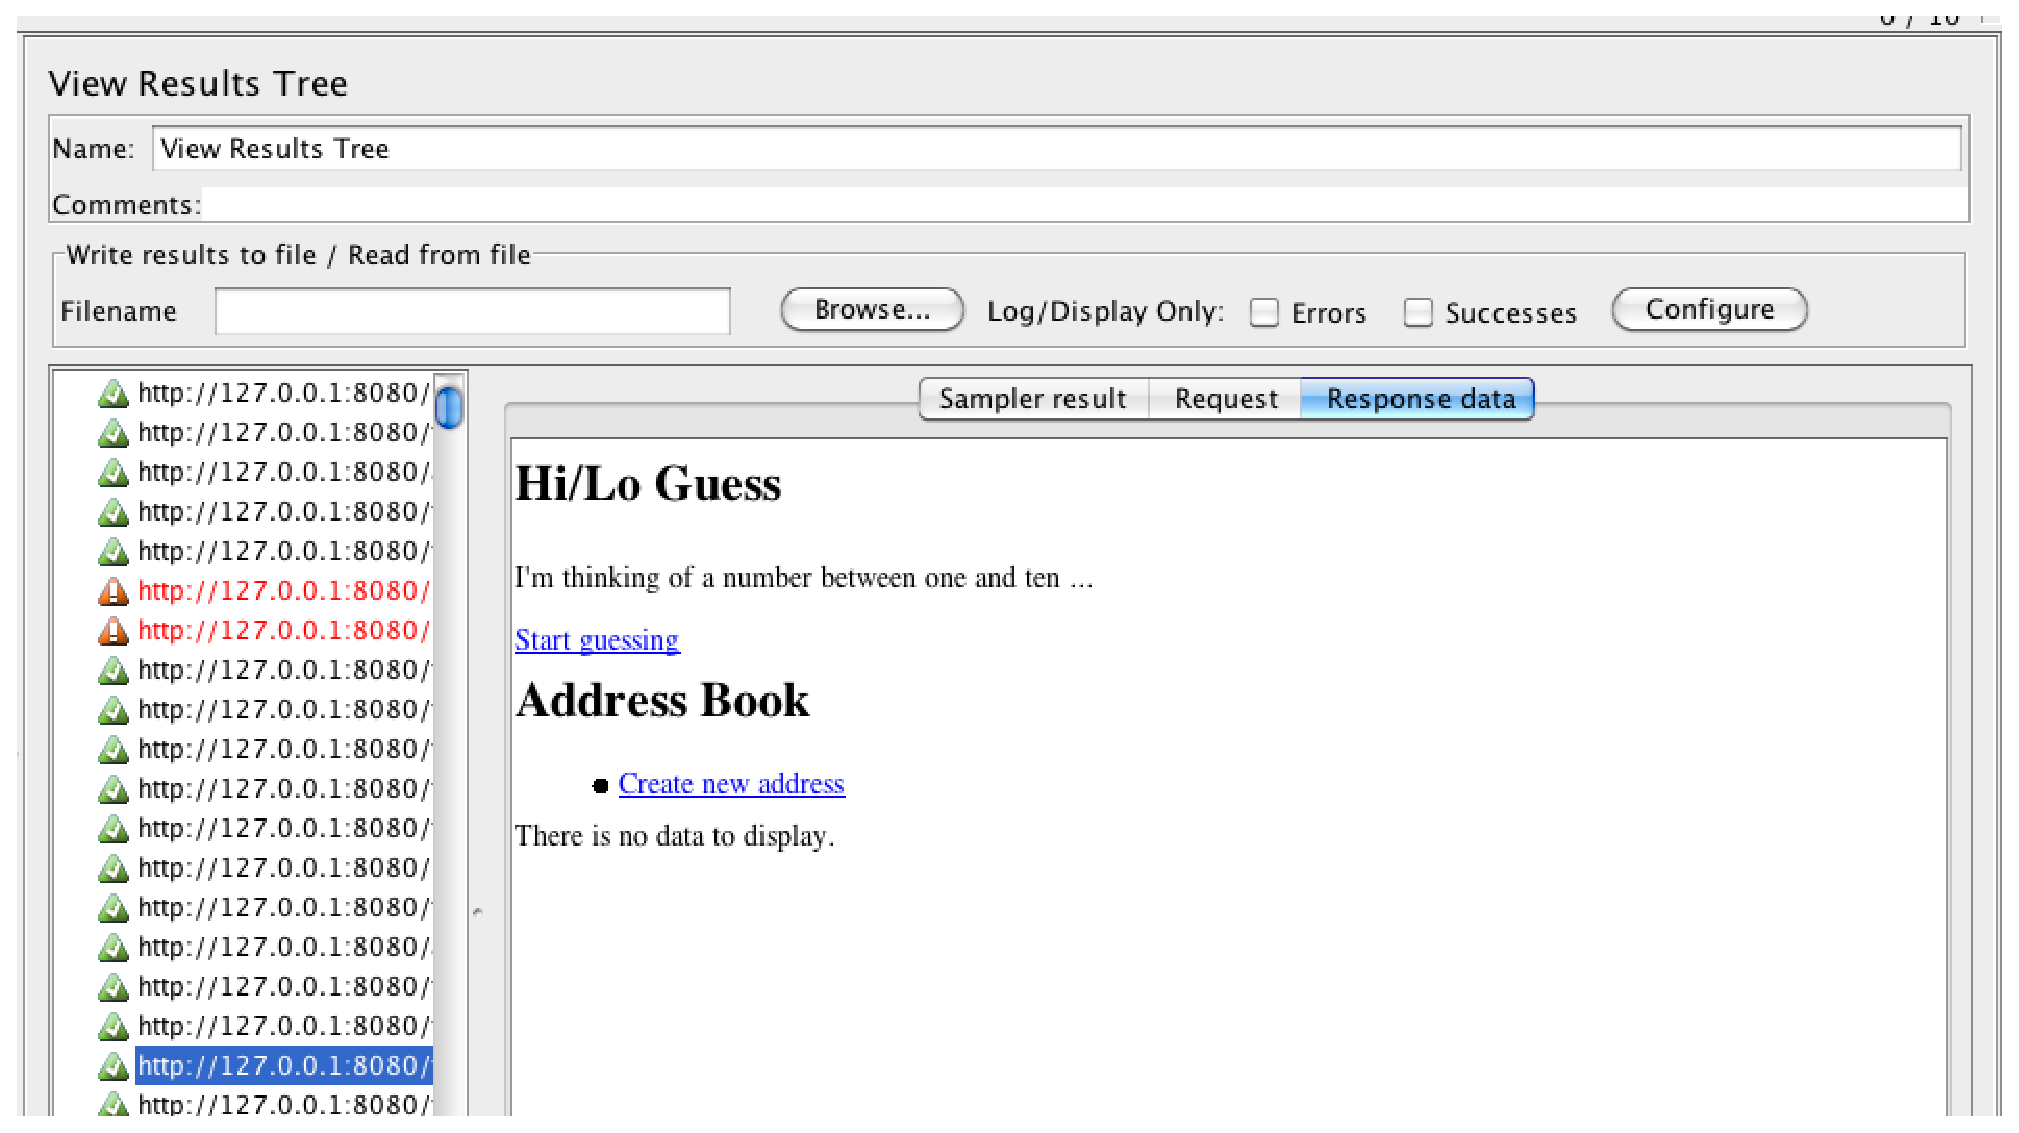
\includegraphics[scale=0.3]{screen/resultTree-Response.eps}	  
  \end{figure}
\end{frame}

\end{document}

%%% Local Variables: 
%%% mode: latex
%%% TeX-master: t
%%% End: 
